% !TeX spellcheck = en_US
\documentclass{standalone}
\usepackage{tikz, float, amsmath }
\usepackage{xcolor}
\usetikzlibrary{patterns}
\usepackage{pgfplots}
\usepackage{pgfplotstable}
\pgfplotsset{width=10cm,compat=1.9}
\usepackage{tkz-euclide}
\tikzset{immagine/.style={above right, inner sep=0pt, outer sep=0pt},
	testo/.style={fill=white, align=center, fill opacity=0.6, text opacity=1, below, font=\sffamily\bfseries\footnotesize}}
	
\definecolor{ForestGreen}{RGB}{34,139,34}
\begin{document}
	
	
	
	
	\begin{tikzpicture}[>=latex]
%\node [immagine] at (0,10)
%{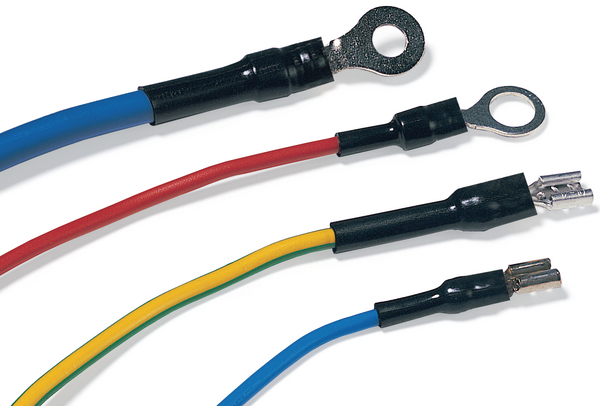
\includegraphics[width=6cm]{heat_tubes}};
%
%\node [immagine] at (8,10)
%{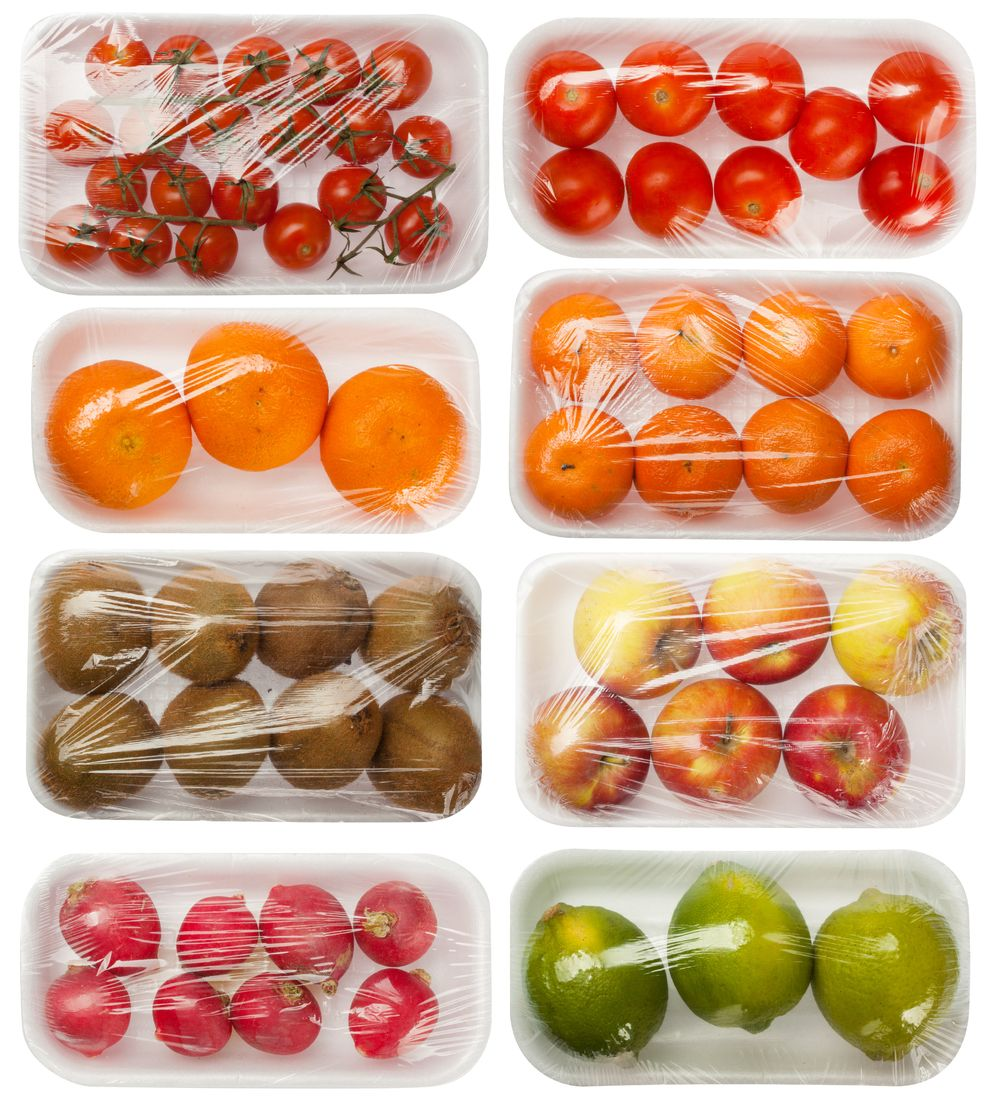
\includegraphics[width=5cm]{film_packaging}};
%
%\node [immagine] at (0,0)
%{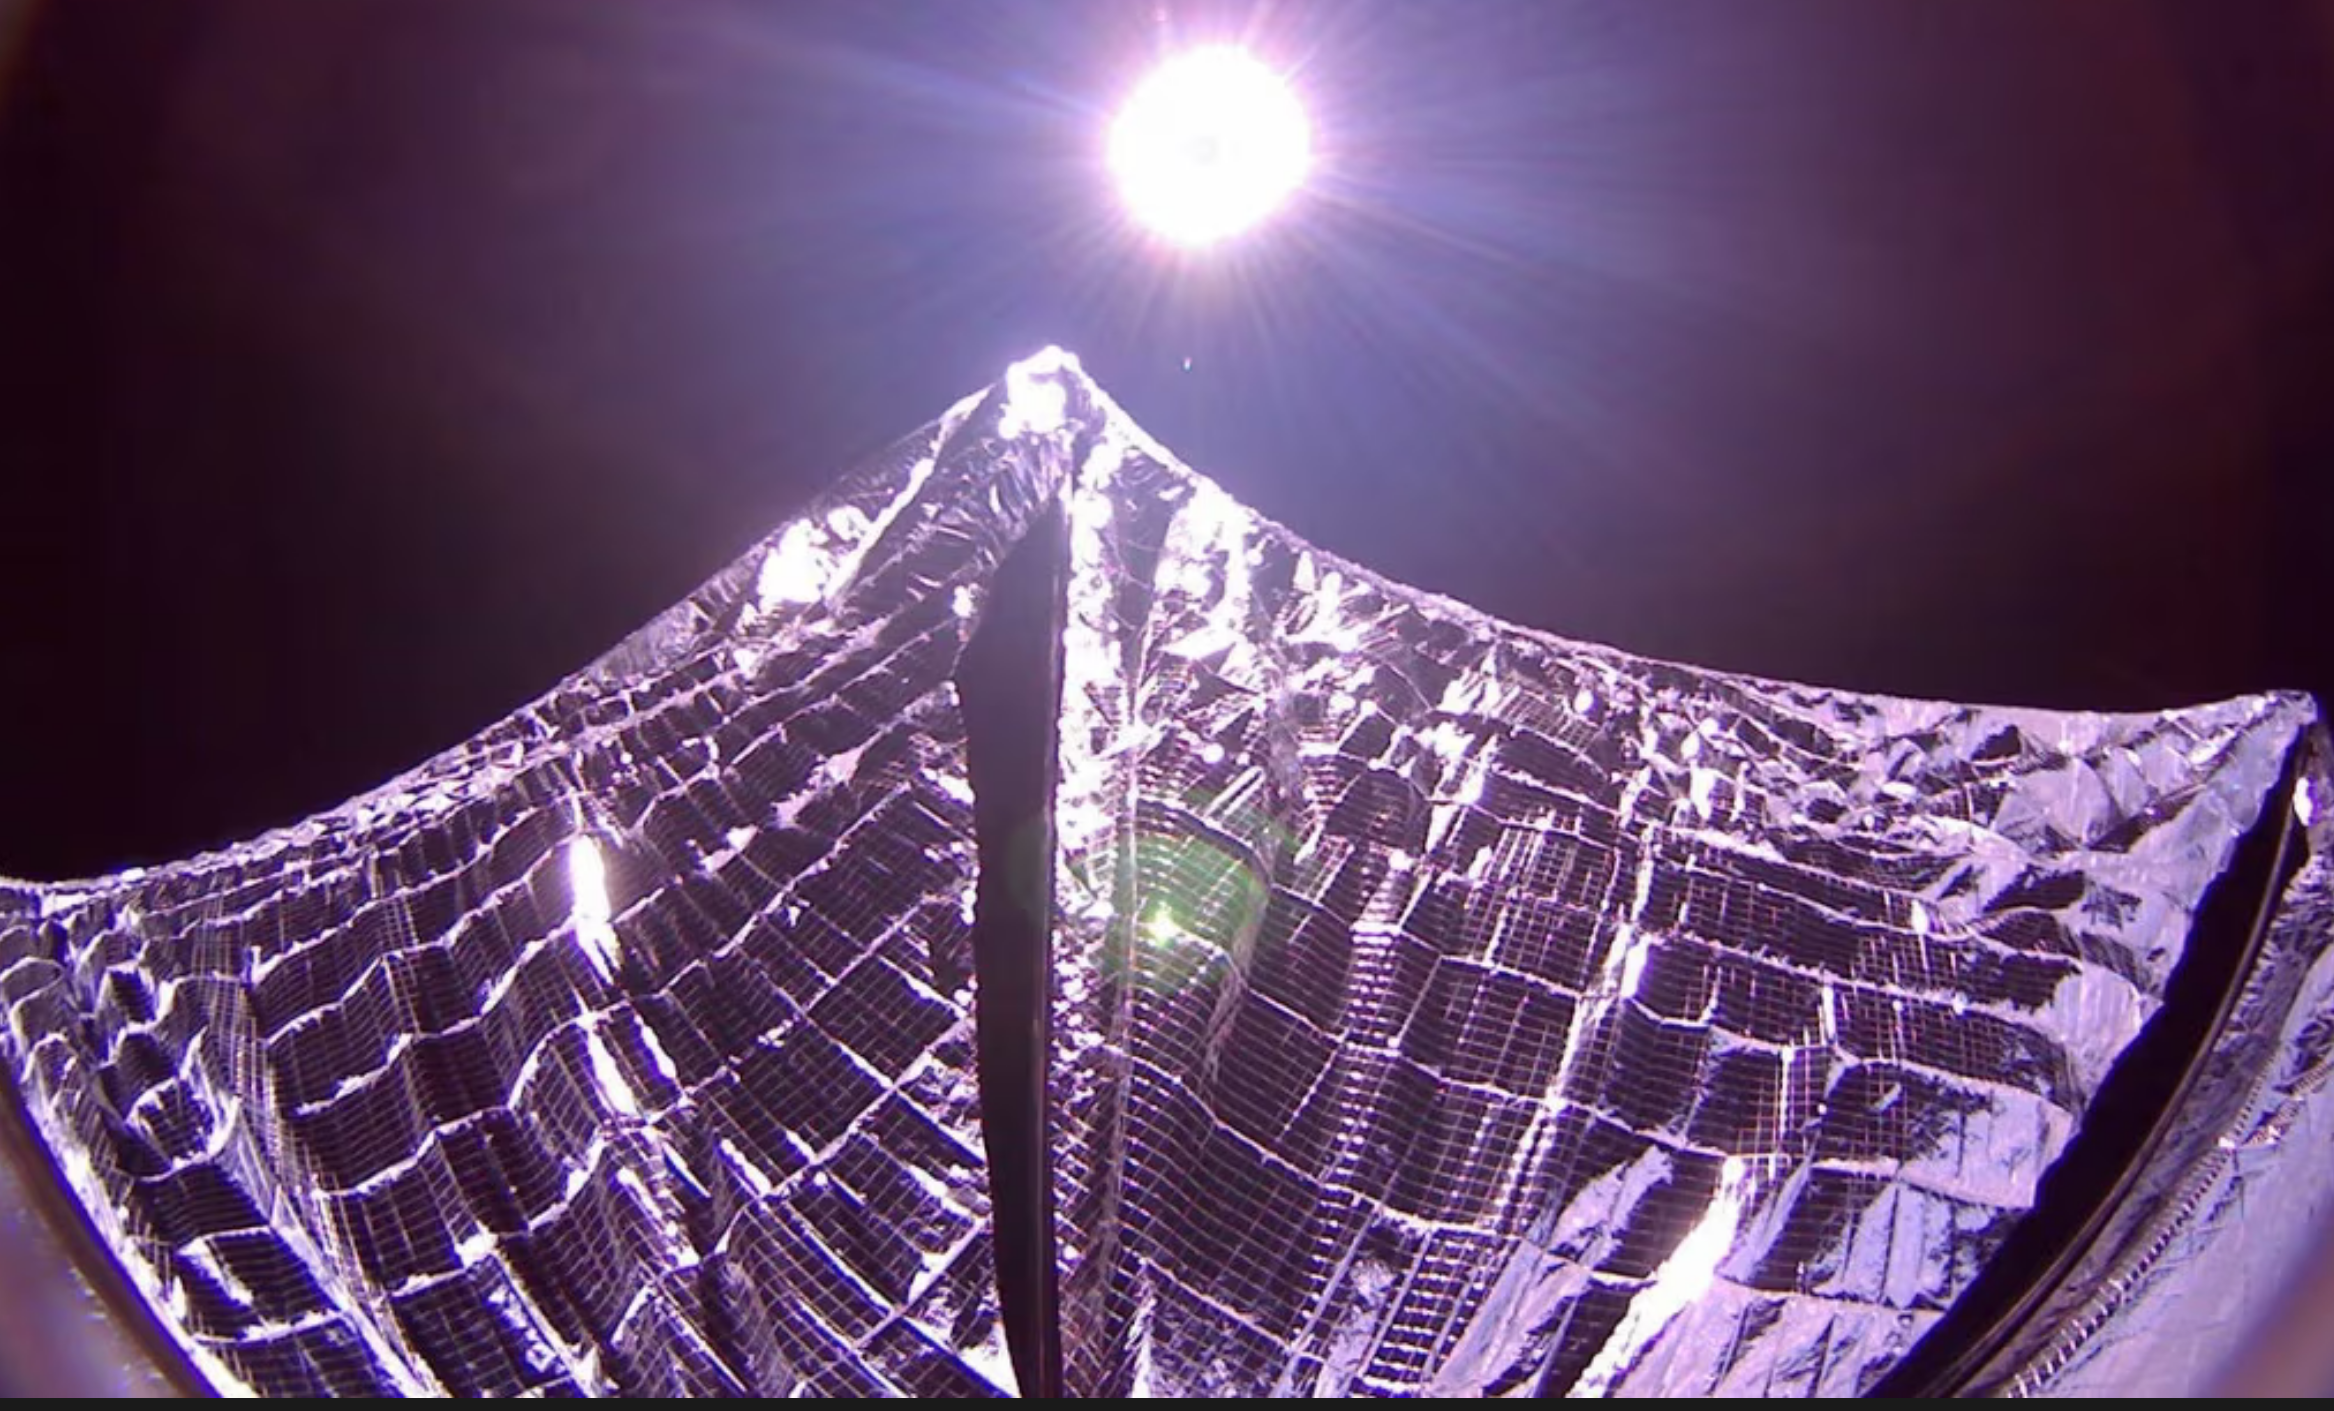
\includegraphics[width=7cm]{sun_sails}};
%
%\node [immagine] at (8,0)
%{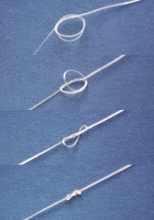
\includegraphics[width=5cm]{surgical_tape}};
%
%\node [immagine] at (0,5)
%{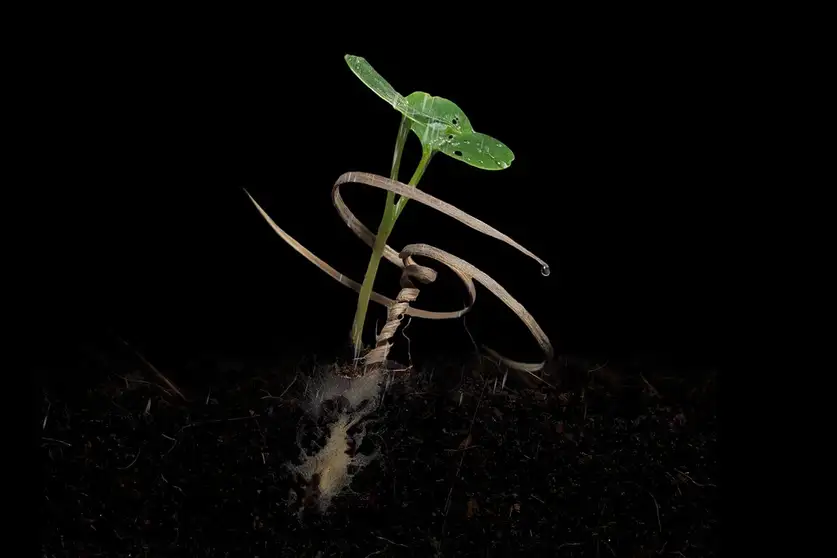
\includegraphics[width=7cm]{artificial_seeding}};


\node [immagine] at (0,0)
{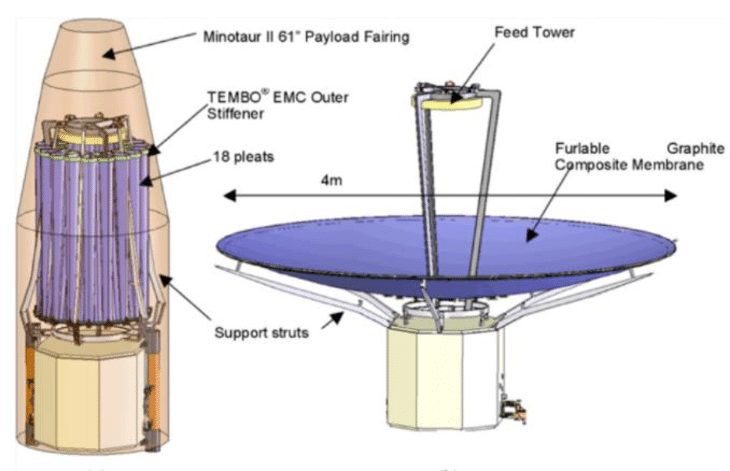
\includegraphics[width=7cm]{SMPC_antennas}};

\node [immagine] at (7,0)
{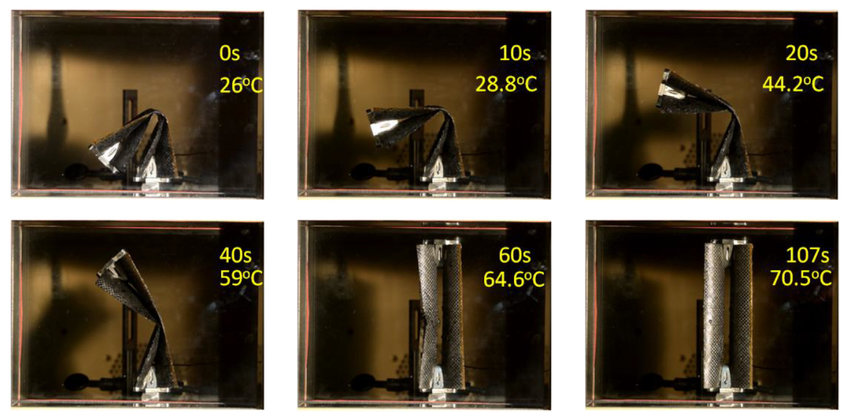
\includegraphics[width=8cm]{SMPC_hinge}};

\node [immagine] at (15,0)
{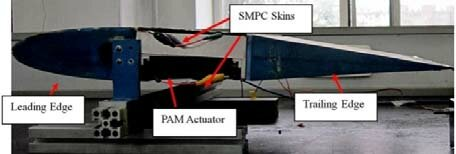
\includegraphics[width=8cm]{SMPC_wing}};

%Help Lines
%\draw [ultra thin, help lines] (0,0) grid (20,5);
%\foreach \x in {0,...,10}
%\draw (\x cm,1pt) -- (\x cm,-1pt) node[anchor=north] {$\x$};
%\foreach \y in {0,...,10}
%\draw (1pt,\y cm) -- (-1pt,\y cm) node[anchor=east] {$\y$};



	\end{tikzpicture}
	
\end{document}
